\documentclass[11pt]{m2pi_v2}
\include{m2pi_standard_commands}
\usepackage{cite}
\usepackage{multicol}
\usepackage{caption}
\usepackage{subcaption}
%\usepackage{hyperref}
\usepackage{xcolor}	 % Required for custom colors
% Define a few colors for making text stand out within the presentation
\definecolor{green}{RGB}{44,85,17}
\definecolor{blue}{RGB}{34,31,217}
\definecolor{brown}{RGB}{194,164,113}
\definecolor{red}{RGB}{255,66,56}
% Use these colors within the presentation by enclosing text in the commands below
\newcommand*{\green}[1]{\textcolor{green}{#1}}
\newcommand*{\blue}[1]{\textcolor{blue}{#1}}
\newcommand*{\brown}[1]{\textcolor{brown}{#1}}
\newcommand*{\red}[1]{\textcolor{red}{#1}}

% Insert custom commands and necessary packages here.

\begin{document}

% A short title is not required, but if needed use:
% \title[short title]{full title}
\title[]{Optimizing marking techniques for mark-recapture studies of mountain pine beetles} 

%% authors listed by last names (add your address/email here)

\author{J. Benesh}\address{Joel Benesh, Department of Mathematics and Computer Science, University of Lethbridge}\email{Joel.Benesh@uleth.ca}
\author{D. Goodsman}\address{Devin Goodsman, Entomologist, Northern Forestry Centre, Natural Resources Canada}\email{goodsman@ualberta.ca}
\author{R. Han}\address{Rachel Han, Department of Mathematics, University of British Columbia} \email{13hanr@gmail.com}
\author{J. Hoepner}\address{Jules Hoepner, Department of Mathematics, University of Victoria}\email{julesihoepner@gmail.com}  
\author{H. Huang}\address{Hui Huang, PIMS Postdoctoral Fellow, University of Calgary} \email{hhduke2014@gmail.com}
\author{M. Ray}\address{Mishty Ray, Department of Mathematics, University of Calgary} \email{mraysamar@gmail.com}

{\thanks{This work was funded by PIMS and Mitacs}}


\vskip 2ex
\maketitle
\begin{center}
\noindent {\small \textsc{Industry mentor:} 
Devin Goodsman, Entomologist, Northern Forestry Centre, Natural Resources Canada \\
}\vspace{1ex}

\noindent {\small \textsc{Academic mentor:}
\\
Hui Huang, PIMS Postdoctoral Fellow, University of Calgary \\
}
\end{center}

\vskip 2ex
\begin{abstract} (Abstract)
%a brief overview of the most important results
\end{abstract}


\vskip 4ex

\section{Introduction}
Since 1990, an outbreak of the mountain pine beetle (\textit{Dendroctonus ponderosae}) has affected over 20 million hectares of forest in western Canada, making it the largest recorded insect outbreak in North American history. These beetles infest trees by laying eggs beneath the outer bark, disrupting nutrient flow and weakening the host tree \cite{aftermath}. Although determining the number of pine beetles is vital in making well-informed environmental decisions, accurately estimating the size of a widespread insect populations can prove highly difficult.
A recent mark-recapture study initiated by Canadian Forest Services attempts to mitigate some of the unknown variation
present in standard population research.

Mark-recapture studies typically involve the application of a harmless indicator to a small number of individuals, which are then released back into the general population. The likelihood of recapturing a marked individual is thus inversely proportional to the size of the population, assuming nearly all of the marked individuals are still alive, and provided no significant immigration into or out of the population has occurred between the release and recapture dates. The NRCAN technique involves covering trees in paper that fluoresces under black light such that the beetles are coated in paper dust as they emerge, thereby allowing the marked beetles to naturally disperse without direct human intervention. Mountain pine beetles emerging from papered trees and control trees were later captured and photographed under black light.

Since manually classifying each image as marked or unmarked can be tedious and prone to error, it would be beneficial to automate the process using machine learning. 
The goal of this project is to develop a new algorithm to identify marked beetles by optimizing pre-existing image classification techniques.
These techniques are discussed in further detail in Section 2, and their implementation is presented in Section 3. In Section 4, the project is summarized and potential improvements to the algorithm are addressed. 





\section{Deep Neural Networks}
Deep learning has been justified by its tremendous empirical success in performing state-of-the-art on various relevant real-life applications such as speech recognition, image recognition, language translation, and as a novel method for scientific computing. It is an approach about realizing complex tasks as the ones mentioned above, by means of highly parametrized functions, called deep artificial neural networks $\mathcal{N}: \mathbb{R}^{d_0}\to  \mathbb{R}^{d_L}$. A classical architecture is the one of feed-forward artificial neural networks of the type
\begin{equation}\label{NN}
\mathcal{N}(x)=\sigma\left(W_{L}^{\top} \sigma\left(W_{L-1}^{\top} \ldots \sigma\left(W_{1}^{\top} x+b_{1}\right) \ldots\right)+b_{L}\right)\,,
\end{equation}
where $L$ is depth of the network,  the function $\sigma$ is a scalar activation function acting component-wisely on vectors, for each layer $\ell=1,\dots,L$, the matrix $W_\ell\in \mathbb{R}^{d_{\ell-1}\times d_{\ell}}$ represents a collection of weights, and the vector $b_\ell$ represents shifts/biases. The neural network \eqref{NN} is then trained to minimize a given loss function (e.g, Mean Squared Error, Cross-Entropy, Kullback-Leibler divergence, or Wasserstein distances) over the parameters (weights and biases) of the network, usually measuring the misfit of input-output information over a given finite number of labeled training samples.

In this report we are going to use Convolutional Neural Networks (CNNs) to solve our image classification problem. However, to train on a very large dataset,  deep CNN models may take a significant amount of time.  A way to bypass this process is to re-use the model parameters from pre-trained top preforming CNN models that were developed for standard computer vision benchmark datasets, such as the ImageNet image recognition tasks. This is the so-called transfer learning. One can see it as  the deep learning version of  "standing on the shoulder of giants".
There are many top-performing models that are available for the basis for image recognition tasks, such as VGG (e.g. VGG19 \cite{simonyan2014very}), GoogLeNet (e.g. InceptionV3 \cite{szegedy2016rethinking}), Residual Network (e.g. ResNet50 \cite{he2016deep}) and EfficientNet (e.g. EfficientNetB0 \cite{tan2019efficientnet}). In the following we are going to focus on the Residual Network and the EfficientNet architectures.

\textit{ResNet50} \cite{he2016deep} is one of the most powerful deep neural networks which has won the ILSVRC 2015 competition because of its fabulous performance. It was proposed to solve the issue of vanishing/exploding gradient phenomenon. The idea is to use the "Residual Block"  (see Figure \ref{res}) to skip connections and after-addition activations. If we denote by $\mathcal{F}(x)=\sigma(W^Tx+b)$ a generic layer of the network, then the residual layer can be described as
\begin{equation}
x^{n+1}=x^n+\mathcal{F}(x^n).
\end{equation}
\begin{figure}
	%\includegraphics[scale=0.4]{ackley3D.pdf}\,
	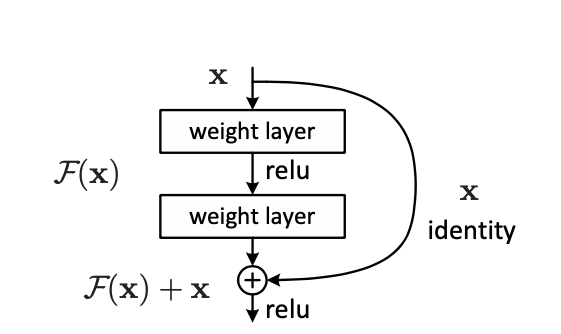
\includegraphics[scale=0.3]{residual.png}\,
	\caption{Residual Block, see\cite{he2016deep}}\label{res}
\end{figure}



\textit{EfficientNet}  was first introduced in \cite{tan2019efficientnet}, since then it has became one of the most efficient models that reaches state-of-the-art accuracy on both ImageNet and common image classification transfer learning tasks. It proposes a compound scaling method  to scale up CNNs in order to obtain better accuracy and efficiency. Unlike conventional approaches that arbitrarily scale network dimensions, such as width, depth and resolution, the EfficientNet uniformly scales each dimension with a fixed set of scaling coefficients. More specifically, it uses a compound coefficient $\varphi$ to uniformly scales network width, depth, and resolution in a principled way:
\begin{equation*}
\begin{aligned}
\text { depth: } d &=\alpha^{\phi} \\
\text { width: } & w=\beta^{\phi} \\
\text { resolution: } & r=\gamma^{\phi} \\
\text { s.t. } & \alpha \cdot \beta^{2} \cdot \gamma^{2} \approx 2 \\
& \alpha \geq 1, \beta \geq 1, \gamma \geq 1\,,
\end{aligned}
\end{equation*}
with $\alpha, \beta$ and $\gamma$ to be determined by grid search. 







\newpage
%%%%%%%%%%%%
\section{Implementation and results} 
\subsection{ResNet50}
In this section we present our transfer training result by using ResNet50.
\begin{figure}
	%\includegraphics[scale=0.4]{ackley3D.pdf}\,
	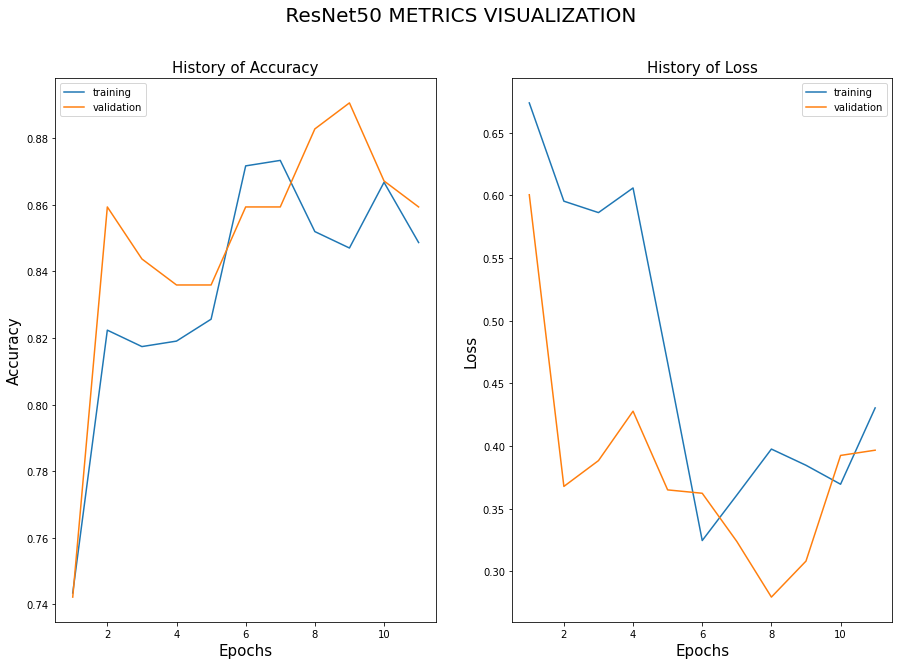
\includegraphics[scale=0.4]{accuresnet.png}\,
	\caption{Accuracy and loss evolution in terms of epochs on training and validation data from ResNet50}\label{resaccu}
\end{figure}
\begin{figure}
	%\includegraphics[scale=0.4]{ackley3D.pdf}\,
	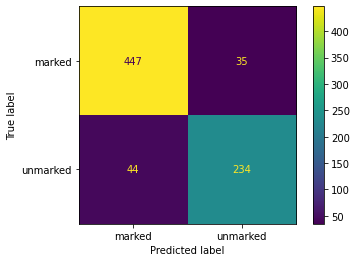
\includegraphics[scale=0.9]{cmresnet.png}\,
	\caption{Confusion matrix for the beetle classifier from ResNet50}\label{rescm}
\end{figure}
Let us use the confusion matrix to test the performance of our classification model obtained from ResNet50. As you can see from Figure \ref{rescm} that we have $447$ true positives (marked beetles were being predicted marked), $35$ false negtives (marked beetles were being predicted unmarked), $44$ false positives (unmarked beetles were being predicted marked), and $234$ true negtives (unmarked beetles were being predicted unmarked). The overall accuracy can be computed by
\begin{equation*}
\mbox{Accuracy}=\frac{\mbox{true positives}+\mbox{true negtives}}{\mbox{total}}=\frac{447+234}{760}\approx 89.6\%.
\end{equation*}



\newpage
\section{Conclusion}






\nocite{*}

\newpage
\bibliographystyle{abbrv}
\bibliography{reference}

\newpage
\end{document}
